\chapter*{Introduction générale}
\addcontentsline{toc}{chapter}{Introduction générale}
\label{chap:introduction}

\section*{Contexte de l'étude}
\addcontentsline{toc}{section}{Contexte de l'étude}

La robotique en essaim s'intéresse à la coopération entre robots relativement simples. Au lieu de confier toute la mission à une seule machine, on mise sur des décisions locales et des échanges limités, d'où émerge un comportement collectif \cite{brambilla2013}. L'idée a des avantages concrets. Le travail se répartit, et le système tient mieux le coup quand un robot tombe en panne ou que d'autres arrivent. On l'utilise surtout pour explorer, surveiller, transporter une charge à plusieurs ou occuper une zone.

Obtenir un résultat collectif précis reste pourtant difficile. Le but peut être de couvrir une région, de garder une formation ou de dessiner une figure, et dans tous les cas chaque robot ne voit qu'une partie de la situation. Les méthodes classiques, celles inspirées du flocking en tête, combinent cohésion, séparation et alignement \cite{reynolds1987,olfati2006}. Elles se comprennent bien. Les adapter se complique dès qu'il faut produire des formes précises, et différentes les unes des autres.

La formation de formes met bien cette difficulté en évidence. Rassembler des robots dans une même zone ne donne ni un cercle, ni une lettre, ni un symbole. Il faut qu'ils se répartissent sur les différentes parties du contour sans trop se rapprocher les uns des autres. Plusieurs travaux ont proposé des contrôleurs décentralisés pour former des courbes et organiser les robots progressivement \cite{hsieh2008,li2019}. Ils montrent l'intérêt du contrôle local. Ils montrent aussi à quel point tout dépend de ce que chaque robot sait.

Dans ce mémoire, le comportement des robots est piloté par un réseau de neurones sur graphes (\emph{Graph Neural Network}, GNN). Les robots en sont les nœuds, leurs communications les arêtes. Tous partagent les mêmes paramètres, et chacun traite ce que lui envoient ses voisins avant de décider de son mouvement. L'intérêt, c'est qu'on peut ainsi apprendre une politique locale tout en gardant une exécution décentralisée \cite{gilmer2017,battaglia2018,tolstaya2020}.

\section*{Problématique}
\addcontentsline{toc}{section}{Problématique}

Un contrôle centralisé organise facilement une formation. Un système central connaît les positions de tous les robots et calcule leurs déplacements. Mais cette solution s'accorde mal avec un essaim, où les communications sont limitées, où le nombre de robots peut varier et où certaines unités tombent en panne. Il faut donc obtenir un comportement collectif sans qu'aucun robot ne possède toutes les informations sur le groupe.

La question principale de ce mémoire est la suivante :

\begin{quote}
\emph{Un réseau de neurones sur graphes utilisant des informations
locales et une consigne commune de forme peut-il apprendre à former
des configurations spatiales et conserver un comportement utile
lorsque des robots tombent en panne ou que la taille de l'essaim
change ?}
\end{quote}

Le caractère décentralisé concerne la décision de mouvement. Chaque robot utilise le même contrôleur et ne parle qu'à ses voisins à portée. La forme à réaliser est fixée avant l'exécution et transmise à l'essaim comme une consigne de mission. Les robots ne la découvrent pas eux-mêmes. Selon la configuration, cette consigne est un identifiant de cible ou une information géométrique locale sur le contour.

L'entraînement, lui, reste centralisé. Il se fait dans un simulateur différentiable, où une perte globale ajuste les poids du réseau. À l'exécution, en revanche, chaque robot décide avec ses informations locales, sans accéder aux positions des robots éloignés.

Cette problématique se décline en quatre questions :

\begin{enumerate}
    \item Le contrôleur appris rapproche-t-il la configuration
    finale de la forme cible, à partir de positions initiales
    aléatoires ?

    \item Les échanges entre voisins améliorent-ils la formation
    par rapport à des règles locales ou à une politique sans
    communication, à information de consigne comparable ?

    \item La politique tient-elle encore quand le nombre de robots,
    et donc de voisins, varie ?

    \item Que devient la qualité de la formation quand des robots
    sont retirés en cours de simulation ?
\end{enumerate}

\newpage

\section*{Hypothèses}
\addcontentsline{toc}{section}{Hypothèses}

Trois hypothèses guident cette étude. Seules des expériences contrôlées pourront les confirmer, ou non.

\begin{enumerate}
    \item Une politique GNN partagée et conditionnée par la forme
    peut réduire l'écart entre les positions des robots et le contour
    cible.

    \item À consigne et ressources comparables, les échanges locaux
    pourraient améliorer la qualité de la formation par rapport à une
    politique sans communication.

    \item Le partage des paramètres permet d'utiliser la politique
    avec différentes tailles d'essaim. Ses performances dépendront
    pourtant de la densité des robots et de la connectivité du
    réseau.
\end{enumerate}

\subsection*{Hypothèses de modélisation et périmètre}

Les expériences du prototype historique se déroulent dans une arène plane, sans obstacle fixe. Chaque robot a une position et une vitesse en deux dimensions. Sa dynamique est simplifiée, la vitesse étant commandée directement. Deux robots communiquent quand leur distance passe sous une portée donnée. Mesures et messages sont supposés exacts, instantanés et sans perte. Un robot en panne est simplement retiré de la simulation et du graphe de communication.

Ces hypothèses simplifient l'étude, mais elles en limitent la portée. Le prototype ignore le bruit des capteurs, les délais de communication, les obstacles, la dynamique réelle des actionneurs et la consommation d'énergie. Aucun essai n'a été mené sur des robots physiques. L'implémentation actuelle prévoit d'étudier certaines perturbations, surtout le bruit des observations et la réduction de la portée de communication, mais les résultats restent à obtenir. Il faudra aussi d'autres expériences pour savoir ce que chaque mécanisme du GNN apporte vraiment.

\section*{Objectifs poursuivis}
\addcontentsline{toc}{section}{Objectifs poursuivis}

L'objectif général est de construire un cadre expérimental reproductible pour étudier le contrôle décentralisé d'un essaim par GNN. Il ne s'agit pas de valider un système physique. On cherche plutôt un environnement où cette approche puisse être étudiée de façon contrôlée.

Les objectifs spécifiques sont les suivants :

\begin{itemize}
    \item développer un simulateur bidimensionnel qui représente les
    positions, les vitesses, les communications entre voisins,
    les limites de l'arène et le retrait de robots ;

    \item constituer un ensemble de formes représentées par des
    nuages de points normalisés, qu'il s'agisse de formes géométriques,
    de chiffres, de lettres ou de nombres ;

    \item développer un contrôleur GNN partagé entre les robots,
    capable de traiter un nombre variable de voisins ;

    \item mettre en place un apprentissage à travers le simulateur,
    en commençant par des formes simples avant de passer aux formes
    symboliques ;

    \item définir un protocole d'évaluation qui mesure la proximité
    de la cible, les collisions, les effets des pannes et le
    comportement quand la taille de l'essaim varie.
\end{itemize}

Le titre déposé parle de « réseaux de neurones cellulaires ». Cette expression renvoie au partage d'une même règle de comportement et à des interactions limitées entre voisins. Or l'architecture réellement implémentée est un GNN à passage de messages sur un graphe dynamique. C'est donc le terme GNN que nous employons dans la suite. Toute modification officielle du titre reste soumise à l'accord de l'encadrement.

\subsection*{Choix du problème étudié}

Nous avons retenu la formation de formes parce qu'elle se prête à un simulateur bidimensionnel tout en posant de vraies difficultés de coordination. Contrairement au simple regroupement, elle oblige les robots à se répartir sur tout le contour cible. On y observe plusieurs aspects du contrôle décentralisé, comme la couverture de la cible, les collisions et la connectivité. La Figure~\ref{fig:schema-formation} en présente les grandes étapes.

\begin{figure}[htbp]
    \centering
    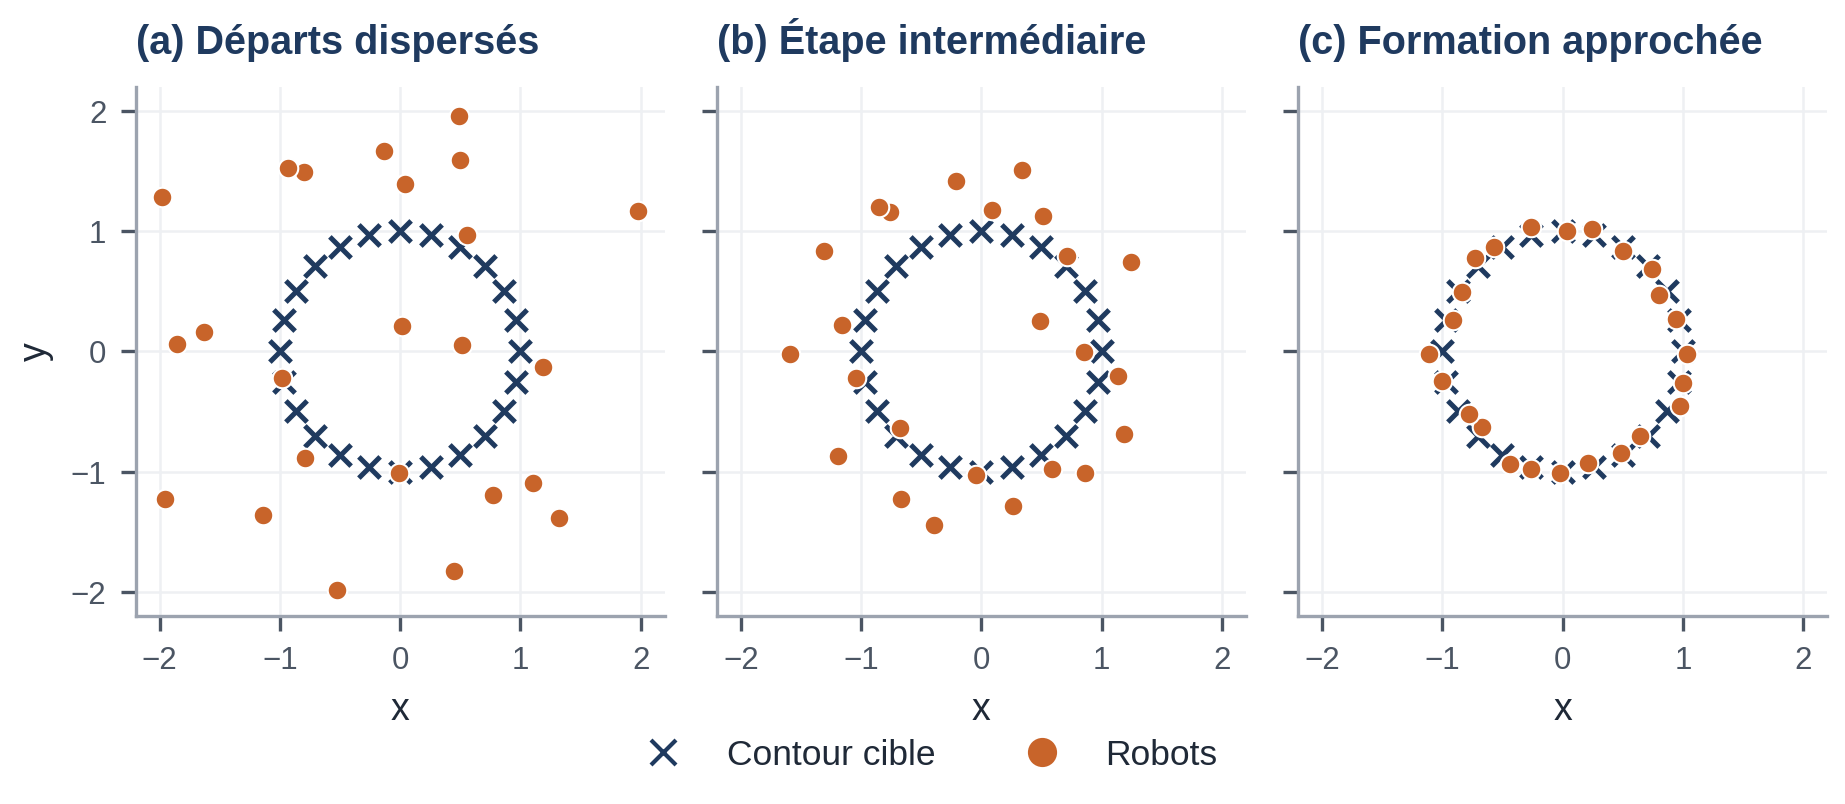
\includegraphics[width=\linewidth,height=.72\textheight,
    keepaspectratio]{images/formation_principle.png}
    \caption[Illustration conceptuelle d'une formation de forme]
    {Illustration conceptuelle d'une formation de forme. À gauche,
    les robots sont répartis aléatoirement. Au centre, ils commencent
    à s'organiser. À droite, ils se rapprochent du contour cible.
    Cette illustration présente le principe général et ne constitue
    pas un résultat du contrôleur appris.}
    \label{fig:schema-formation}
\end{figure}

Le cercle vient en premier, car son contour est régulier et se représente facilement par un nuage de points. Chiffres et lettres suivent, avec leurs angles, leurs segments et leurs contours moins réguliers. Nous ne cherchons pas à reconnaître les symboles. Il s'agit seulement de voir si les robots en reproduisent la géométrie. Une lettre formée à peu près ne veut pas dire que le système en comprend le sens.

La consigne commune compte beaucoup. La forme cible est connue avant le début de la simulation, mais chaque robot décide de son mouvement avec ses propres informations et celles de ses voisins. Aucun système central ne lui envoie les positions de tout l'essaim. C'est ce point précis qui rend le contrôleur décentralisé.

\subsection*{Critères de réussite}

Une animation convaincante à l'œil ne prouve pas que la formation est réussie. Les robots doivent s'approcher du contour cible et en couvrir les différentes parties, avec des commandes bornées et peu de collisions.

La reproductibilité compte aussi. Une même configuration et une même graine aléatoire doivent redonner le même scénario. Et il faut plusieurs graines, pour ne pas s'appuyer sur une seule simulation favorable.

La robustesse s'évalue à part. Qu'un modèle fonctionne avec plus de robots qu'à l'entraînement ne prouve pas qu'il généralise. Retirer des robots n'est qu'une panne simplifiée. Les capteurs défaillants, ou les robots immobilisés qui restent dans l'environnement, demanderont d'autres études.

\section*{Méthodes et techniques utilisées}
\addcontentsline{toc}{section}{Méthodes et techniques utilisées}

Tout commence par un simulateur fiable. Il doit représenter correctement les distances entre robots, les communications et l'évolution des positions, sans quoi les résultats seraient faussés, quelle que soit la qualité du modèle appris. Une règle locale de regroupement sert de première référence : la simulation doit se comporter comme elle le prédit.

Les formes cibles sont ensuite représentées par des nuages de points. Une forme devient alors un ensemble de positions à couvrir, et non une image à reconstruire pixel par pixel. On peut ainsi comparer la distribution des robots à celle du contour cible. Le nombre de robots disponibles limite quand même le niveau de détail reproductible.

Vient l'apprentissage du contrôleur GNN. Les robots partent de positions initiales variables et partagent les mêmes paramètres. Le contrôleur doit donc faire face à des situations très différentes pendant la simulation. Son comportement ne s'évalue correctement que sur des scénarios variés, avec plusieurs graines aléatoires.

Les résultats se lisent enfin à partir de plusieurs éléments. La courbe de perte renseigne sur l'apprentissage, les visualisations montrent la formation obtenue et les mesures calculées sur plusieurs épisodes donnent la variabilité des performances. Aucun de ces éléments ne suffit seul. Une belle animation ne vaut pas une validation expérimentale.

\section*{Contribution de l'étude}
\addcontentsline{toc}{section}{Contribution de l'étude}

Ce travail propose un cadre expérimental qui réunit la représentation des formes par nuages de points, un contrôleur GNN partagé et un protocole pour rejouer les simulations et analyser les trajectoires enregistrées. Il veut faciliter l'étude du contrôle décentralisé. Il ne prétend pas établir une supériorité générale des GNN sur les autres méthodes.

Les résultats numériques disponibles viennent du prototype historique. Avant de tirer des conclusions plus générales, il faudra entraîner et valider l'implémentation actuelle.

\section*{Plan sommaire et subdivision du travail}
\addcontentsline{toc}{section}{Plan sommaire et subdivision du travail}

Après cette introduction, le mémoire compte quatre chapitres. Le premier pose les notions de base de la robotique en essaim et du contrôle local. Le deuxième passe en revue les méthodes existantes et les travaux sur la formation de formes. Le troisième décrit la méthodologie, avec le simulateur, les formes cibles, le contrôleur et la procédure d'apprentissage. Le quatrième présente l'implémentation et les résultats du prototype historique, avec leurs limites. Une discussion et une conclusion générale terminent le travail.

La Figure~\ref{fig:experimental-pipeline} résume la chaîne expérimentale. L'apprentissage utilise une perte globale dans le simulateur. Ensuite, chaque robot applique la politique partagée avec ses observations locales, les informations de ses voisins et la consigne de mission.

\begin{figure}[htbp]
    \centering
    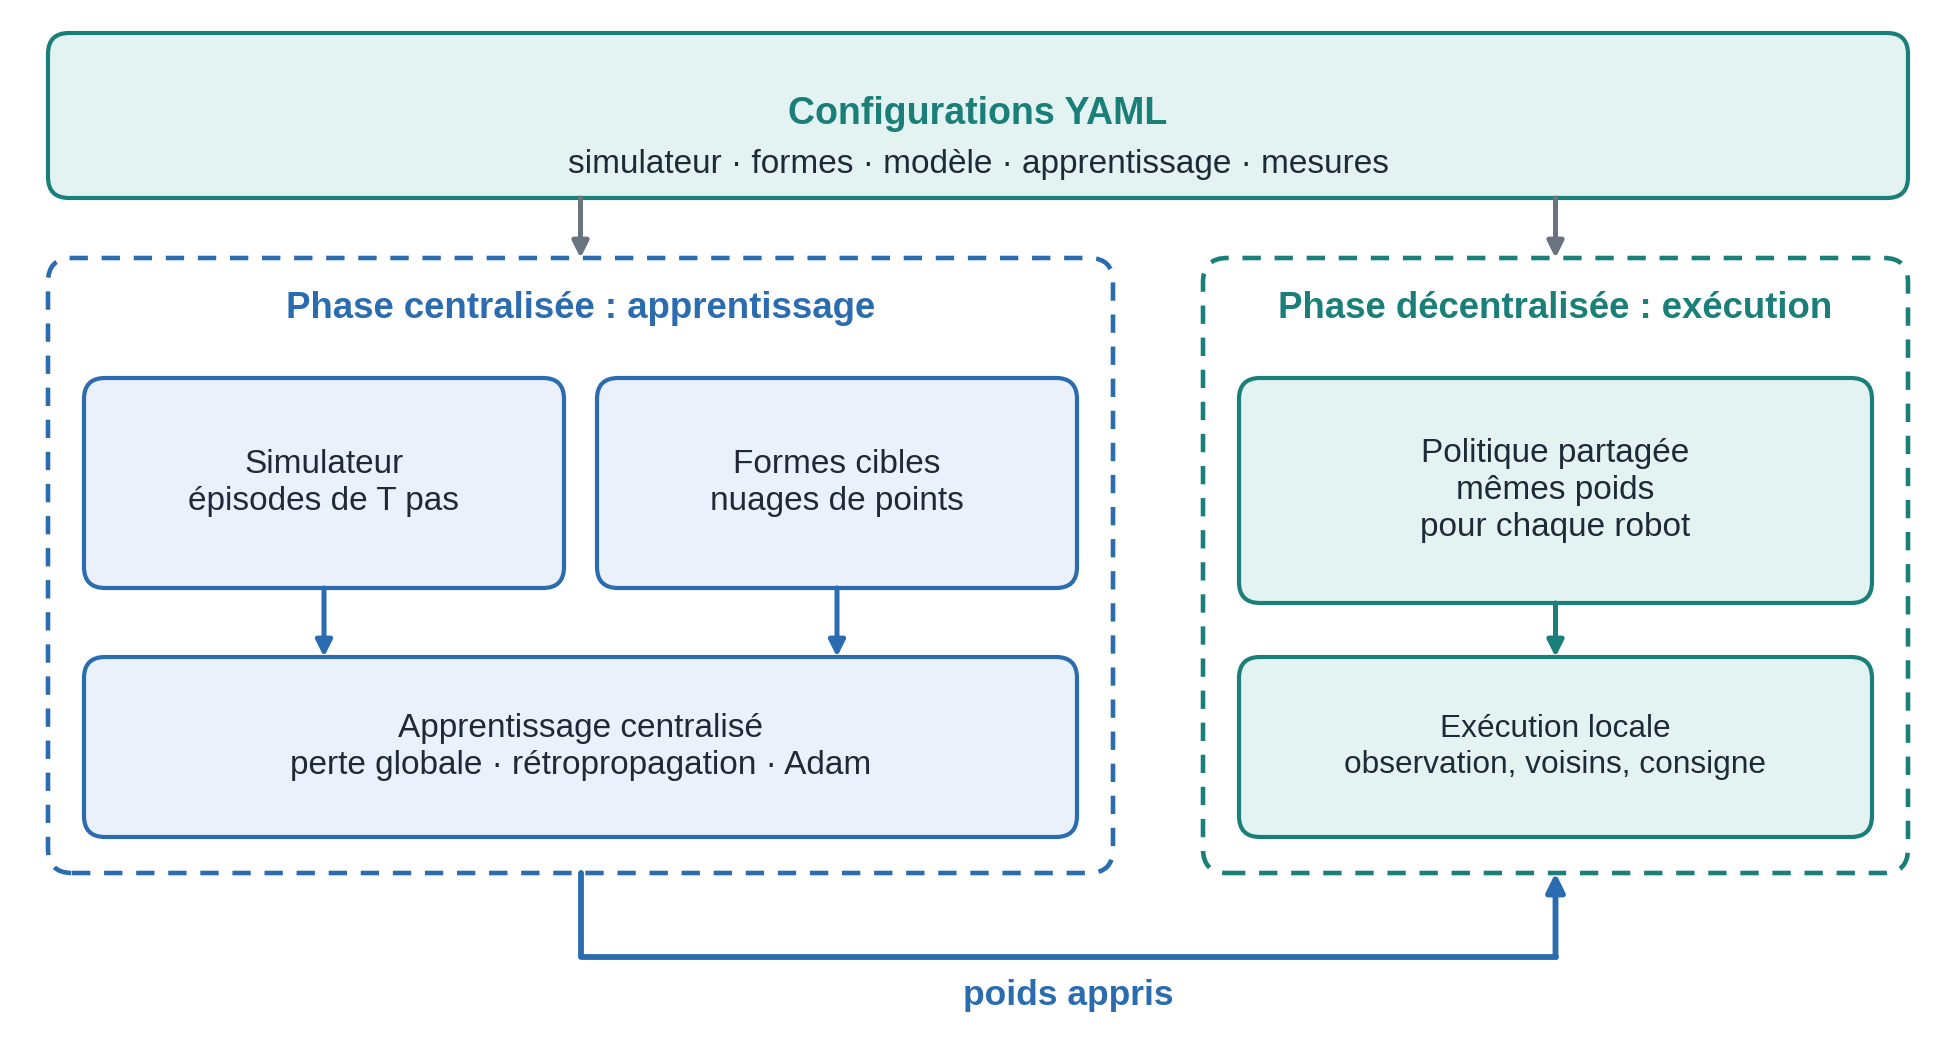
\includegraphics[width=\linewidth]{images/experimental_chain.png}
    \caption[Vue d'ensemble de la chaîne expérimentale]
    {Vue d'ensemble de la chaîne expérimentale. L'apprentissage
    repose sur une perte globale. Pendant l'exécution, chaque robot
    utilise la politique partagée à partir de ses informations
    locales, de ses voisins et de la consigne de mission.}
    \label{fig:experimental-pipeline}
\end{figure}